\documentclass[11pt]{scrartcl}
\usepackage[utf8]{inputenc}
\usepackage[german]{babel}
\usepackage{amsmath}
\usepackage{amsfonts}
\usepackage{amssymb}
\usepackage{bigstrut}
\usepackage{graphicx} 
\usepackage{listings}
\usepackage{xcolor}
\usepackage{alltt}
\usepackage[colorlinks=true,linkcolor=darkgray]{hyperref}

\begin{document}

\title{Entwicklung von Anwendungen mit dem RedPitaya}
\author{Paul Hill}
\date{28.05.2016}

\maketitle
\tableofcontents
\newpage

\section{Vorwort und Überblick}
Diese Dokumentation soll den Einstieg in das Entwickeln von Anwendungen, insbesondere von Web-Anwendungen für den RedPitaya, erleichtern. Sie bezieht sich auf die OS-Version 0.95 (April 16), einige Dinge mögen sich mit kommenden Versionen also ändern. Neben C, kann der RedPitaya auch über andere Wege \grqq programmiert\grqq~werden (zb Matlab), auf welche ich hier aber nicht näher eingehen werde. \\
Wenn Sie einen Fehler gefunden oder sonstige Fragen oder Vorschläge haben, können Sie mich gerne unter paul.hill@stud.uni-heidelberg.de kontaktieren.\\
 
Für einen guten Überblick sei zunächst auf die RedPitaya-Wiki in der \href{http://wiki.redpitaya.com/index.php?title=Main_Page}{aktuellen\footnote{http://wiki.redpitaya.com/index.php?title=Main\_Page}} und der 
\href{http://wiki.redpitaya.com/index.php/OLD_OS_Main_Page}{alten Version\footnote{http://wiki.redpitaya.com/index.php/OLD\_OS\_Main\_Page}} verwiesen. 
In letzterer finden sich ein Benutzerhandbuch und eine Entwicklerdokumentation, die als erster Einstieg in die Materie genutzt werden sollten.

\section{Installation und Vorbereitung der Entwicklungsumgebung}
Nachdem die SD-Karte wie in der Wiki beschrieben vorbereitet wurde, ist der RedPitaya bereits einsatzbereit. \\
Möchte man selber Anwendungen entwickeln, müssen jedoch zunächst noch einige Vorbereitungen getroffen werden. Der Aufbau der Entwicklungsumgebung ist vom verwendeten Betriebssystem des Arbeitsrechners abhängig, eine Anleitung findet sich auch hier in der Wiki. \\

Als erster Schritt sollte die \href{https://github.com/RedPitaya/RedPitaya}{Git-Repository\footnote{https://github.com/RedPitaya/RedPitaya}} des Red-Pitaya Projektes heruntergeladen werden, diese enthält alle notwendigen Quelldateien der bestehenden Anwendung (samt dem NGINX-Modul und dem Verilog-Projekt für den FPGA) und Beispiele, die für die Entwicklung benötigt werden. Im Folgenden müssen noch diverse Software-Pakete (Linaro Toolchain, Xilinx, ..) installiert werden. Hier kann nach der Anleitung der Wiki vorgegangen werden, es sollten aber unbedingt auch die entprechenden README-Dateien aus der Repository gelesen werden! Bei Abweichungen sollte man den READMEs folgen, da die Informationen in der Wiki womöglich veraltet sind. Achten Sie auch darauf, dass Sie die richtige Version des Cross-Compilers installieren, denn diese muss zum benutzten RedPitaya passen (man unterscheidet zwischen hardfloated \grqq hf\grqq~und softfloated). An dieser Stelle sei darauf hingewiesen, dass es beim Vorbereiten der IDE zu Problemen (d.h insbesondere zu Fehlern bei der Kompilierung) kommen kann, die den Prozess stark hinauszögern können. In solchen Fällen sollte man sich vergewissern, streng nach den Readme-Dateien vorgegangen zu sein und notfalls noch einmal von vorne beginnen. \\

Kommt man nicht weiter, ist als generelle Anlaufstelle das \href{http://forum.redpitaya.com/}{RedPitaya Forum\footnote{http://forum.redpitaya.com/}} zu nennen, in dem man kompetente Hilfe findet.\\

Da die Vorbereitung der Entwicklungsumgebung mitunter mühselig ist, kann bei kleineren Projekten auch direkt auf dem RedPitaya gearbeitet werden. Per ssh-Verbindung können Quelldateien hier direkt mit gcc kompiliert werden. Eine ausführlichere Beschreibung findet sich in der Wiki.\\
 

\section{Die RedPitaya Api}
Die standardmäßig auf dem RedPitaya enthaltenen Webanwendungen kommunizieren über in C geschriebene Module direkt mit dem FPGA, da bei deren Entwicklung noch keine Api bereitstand. Mittlerweile exisitiert allerdings eine solche Api, die diese Kommunikation abstrahiert und den Zugriff auf die auf dem FPGA implementierten Funktionalitäten erheblich erleichtert (für die Funktionalität der PIDs muss aber nach wie vor auf ein entsprechendes C-Modul zurückgegriffen werden, welches jedoch sehr überschaubar ist).
Für die Api exisitiert eine \href{http://libdoc.redpitaya.com/rp_8h.html}{Dokumentation\footnote{http://libdoc.redpitaya.com/rp\_8h.html}} und es bestehen einige Beispiele in der Repository (\grqq Examples/C\grqq ).\\
Die Beispiele und die Dokumenation sind an sich sehr instruktiv, deswegen soll an dieser Stelle nicht allzu sehr auf deren Funktionalität eingangen werden. Es sei doch auch darauf hingewiesen, dass es an manchen Stellen Unstimmigkeiten in der Dokumenation und den Beispielen gibt. Bei Schwierigkeiten sollte man sich den Quellcode (\grqq api/rpbase/src/\grqq ) der API direkt anschauen (notfalls auch den Verilog-Code). \\

Programme, die die Api benutzen, müssen, wenn sie in einer Shell aufgerufen werden, mit 'LD\_LIBRARY\_PATH=/opt/redpitaya/lib' gestartet werden.

\subsection{Oszilloskop-Funktion}
Insbesondere das Acquirieren von Samples über den (Fast-) ADC, stellte sich als schwieriger heraus, weswegen dies nun genauer betrachtet werden soll.\\
Schauen Sie sich dazu das Programm \grqq acq\_api\_test\grqq~an. In dem gleichnamigen Projektordner (in meinem Archiv) liegt eine Txt-Datei mit einer Ausgabe des Programms. Beide Dateien finden Sie auch im Anhang.\\

Intern werden die gelesenen Samples in einem zirkulären Buffer (je Channel) der Länge 16384 gespeichert. Der Index des aktuellsten Samples steht in dem sogenannten \grqq Write Pointer\grqq. Die Samples hinter dem Write Pointer sind am ältesten und werden als nächstes überschrieben werden.\\
Mit dem Befehl 'rp\_AcqStart()' wird mit dem Einlesen von Samples begonnen. Wird nun eine Triggerquelle mit 'rp\_AcqSetTriggerSrc(..)' gesetzt, ist das \grqq Oszilloskop\grqq~scharf gestellt. Wird der Trigger ausgelöst, wechselt der Triggerstatus zu \grqq triggered\grqq . Nachdem die zuvor mit 'rp\_AcqSetTriggerDelay(..)' angebene Samplezahl (+interner Offset!) acquiriert wurde, wird die Triggerquelle auf \grqq disabled\grqq~gesetzt und der Triggerstatus wechselt wieder zu \grqq waiting\grqq. Nun werden keine weiteren Samples mehr eingelesen und es kann mit dem Auslesen der Daten begonnen werden. Ob man den internen Offset für das Triggerdelay umgehen sollte, hängt von der Art der Anwendung ab. Setzt man das Triggerdelay auf 0, sorgt der interne Offset (von + 16384/2) dafür, dass genauso viele \grqq Pre-Trigger-\grqq~wie \grqq Post-Trigger-Samples\grqq~zur Verfügung stehen. Dies kann zB bei einer Oszilloskop ähnlichen App von Nutzen sein.\\
Es ist wissenswert, dass 'rp\_AcqReset()' das Einlesen von Samples nicht beendet (es werden nur die gesetzten Parameter zurückgesetzt)! Im obigen Programm würde ein Aufruf von 'rp\_AcqStart()' am Ende der main-Funktion dazu führen, dass bei einem erneuten Programmstart bereits vor 'rp\_AcqStart()' Samples acquiriert werden würden.\\ 
Desweiteren kann es, je nach verwendeter Triggerquelle (zb \grqq AWG\grqq), Probleme mit dem Triggern geben. Dabei mag es helfen, einen 'sleep'-Befehl zwischen 'rp\_AcqStart()' und 'rp\_AcqSetTriggerSrc()' zu setzen (siehe z.B. \grqq Laser Stabilizer\grqq -App).

\subsection{Kompilierung (Ubuntu)}
Zum Kompilieren der App werden Makefiles verwendet. Beispiele dafür finden sich in den Projektordnern in \grqq Examples/C/\grqq~in der Repository. Eine typische Makefile sieht dann bspw. so aus:
\lstset{breaklines=true, showstringspaces=false, keywordstyle=\bfseries\color{purple},
commentstyle=\itshape\color{green},
identifierstyle=\color{blue},
stringstyle=\color{orange},basicstyle=\footnotesize\ttfamily}

\lstinputlisting[caption={Makefile},captionpos=t,language=bash]{../lock/Makefile}

Im jeweiligen Verzeichnis kann das Programm dann im Terminal mit \\'make CROSS\_COMPILE=arm-linux-gnueabihf- all' (hardfloated Version) kompiliert werden. Hat man zuvor das Skript \grqq settings.sh\grqq~(Repository) ausgeführt, reicht der Befehl 'make all' aus. Vor dem erneuten Kompilieren kann es notwendig sein, zuerst alle zuvor bei der Kompilierung erzeugten Datein zu löschen ('make clean').

\section{Web-Apps}
Eine wichtige Funktionalität des RedPitayas sind die sogenannten Web-Apps:\\
Eine Web-Oberfläche, die über einen Browser zugänglich ist, dient als graphische Schnittstelle zum Nutzer, sodass dieser auf sehr einfachem Wege Einstellungen/Befehle an der laufenden Anwendung vornehmen kann und direkt eine visuelle Darstellung der generierten Daten erhält. Dazu läuft auf dem RedPitaya der modularisierbare Web-Server NGINX. Das entsprechende Modul für die Webanwendungen ist in C geschrieben und findet sich \href{https://github.com/RedPitaya/RedPitaya/tree/master/Bazaar/nginx/ngx_ext_modules/ngx_http_rp_module}{hier\footnote{https://github.com/RedPitaya/RedPitaya/tree/master/Bazaar/nginx/ngx\_ext\_modules/ngx\_http\_rp\_module}}. So werden HTTP-Anfragen spezieller Art vom Web-Server nicht \grqq wie gewohnt\grqq~verarbeitet, sondern über das Modul an die derzeit laufende Web-Anwendung weitergeleitet. Selbige besteht dann aus einem serverseitigen Programm (ebenfalls in C), das einige Funktionen (\grqq entry points\grqq ) implementieren und als shared-object Datei kompiliert werden muss. Innerhalb dieses C-Programms kann dann wie gewohnt (zB mit der Api) gearbeitet werden.\\
Der Sourcecode der bereits existierenden Webanwendungen findet sich in der Repository unter \grqq apps-free\grqq~in den jeweiligen Projektordnern.\\
Auch die Wiki bietet einen Überblick über \href{http://wiki.redpitaya.com/index.php?title=Red_Pitaya_WEB_application_structure_detailed_overview}{Web-Apps\footnote{http://wiki.redpitaya.com/index.php?title=Red\_Pitaya\_WEB\_application\_structure\_detailed\_overview}}.\\
Für die Entwicklung kann es sehr hilfreich sein, den Traffic der Anwendungsoberfläche einsehen zu können. Eine solche Funktionalität sollte in nahezu jedem Browser vorhanden sein.\\
Eine sehr simple \grqq Hello World!\grqq -Anwendung findet sich im Ordner \grqq web-apps/test\grqq~in meinem Archiv.

\subsection{Aufbau, benötigte Dateien und Installation}
Eine Web-App besteht zunächst aus einem Ordner mit einem eindeutigen Namen, der App-Id (zb \grqq pid+gen\grqq ). Dazu werden mindestens fünf weitere Dateien benötigt:
\begin{itemize} 
\item fpga.conf ..Verweis auf die zu verwendende FPGA-Datei. Falls keine eigene verwendet werden soll, zb '/opt/redpitaya/fpga/fpga\_0.94.bit' (Version!)
\item index.html ..Die HTML-Datei für die Weboberfläche
\item controllerhf.so ..Die eigentliche Anwendungsdatei, die vom Webserver angesprochen wird (Version für hardfloated Gerät)
\item info/icon.png ..Ein Icon für die Weboberfläche
\item info/info.json ..Enthält Metainformation im JSON-Format, zb:
\begin{lstlisting}
{
    "name": "Laser Stabilizer",
    "version": "0.94-BUILD_NUMBER",
    "revision": "REVISION",
    "description": "Scan & PID Controller for laser stabilization."
}
\end{lstlisting}
\end{itemize}
Es können natürlich auch zusätzliche Dateien (zb css, js, ...) verwendet werden.\\
Zum Installieren der App muss der Ordner mit den obigen Dateien in das Verzeichnis \grqq /opt/redpitaya/www/apps/\grqq~des RedPitayas kopiert werden (gegebenenfalls muss der Ordner 'appId' erst noch erstellt werden).

\subsection{Controller-Datei und Kommunikation zwischen Server- und Clientseite}
Auf der Clientseite können mittels Ajax HTTP GET- und POST-Anfragen an den Server gestellt werden. Bei entsprechender URL, werden sie von NGINX über das NGINX-RedPitaya-Modul an unsere controller-Datei weitergegeben. Es stehen im wesentlichen die folgenden vier Anfragen zur Verfügung ('root\_url ' ist der jeweilige Hostname des RedPitayas):
\begin{itemize}
\item root\_url + '/bazaar?start=' + app\_id ..Initialisiert die Anwendung, app\_id muss gleich dem Namen des Projektordners sein
\item root\_url + '/bazaar?start=' ..Stoppt die Anwendung
\item POST root\_url + '/data' ..Zum Senden der aktuellen Parametereinstellungen. Die Antwort enthält die aktuellen, serverseitigen Parameter. Die Daten werden dabei im JSON-Format übertragen. Eine typische Antwort kann bspw. so aussehen:
\begin{lstlisting}
{
  "app":{
	  "id":"stabilizer"
  },
  "datasets":{
	  "params":{
		  "op_mode":0,
		  "xmin":25,
		  "xmax":75,
		  "trig_delay":1145.469727,
		  ...
	  }
  },
  "status":"OK"
}
\end{lstlisting}
\item GET root\_url + '/data' ..Fordert den Server dazu auf, die aktuellen \grqq Signale\grqq~und Parameter zu schicken. Die Antwort enthält entsprechende Signale und Parameter. Bei den Signalen handelt es sich um zwei zweidimensionale Arrays von jeweils max. 2048 Elementen. Üblicherweise enthält jedes der Arrays die Messergebnisse für je einen der Analogeingänge, wobei ein Messpunkt aus einem Zeit- und Spannungswert besteht. Die Signale werden ebenfalls im JSON-Format beschrieben, eine typische Antwort könnte so aussehen:
\begin{lstlisting}
{
  "app":{
	  "id":"stabilizer"
  },
  "datasets":{
	  "g1":[{"data":[[0.0000,-0.0247],[25.0655,-0.0248],...]}, {"data":[[0.0000,-0.0159],[25.0655,-0.0159],...]}],
	  "params":...
  }
  "status":"OK"
}
\end{lstlisting}
\end{itemize} 

Intern (NGINX-RP-Modul) spielt die folgende Struktur eine zentrale Rolle:
\begin{lstlisting}
typedef struct rp_app_params_s {
    char  	*name;
    float 	value;
    int 	fpga_update;
    int    	read_only;
    float  	min_val;
    float	max_val;
} rp_app_params_t;
\end{lstlisting}
Diese Struktur repräsentiert genau einen Parameter, wobei nur die ersten beiden Variablen für die Kommunikation mit der Clientseite verwendet werden. Die restlichen vier Variablen sind für den Gebrauch innerhalb der Controller-Datei reserviert. Die aus der JSON-Anfrage geparsten Parameter werden zur weiteren Verwendung in einem Array gespeichert. Z.B.:
\begin{lstlisting}
rp_app_params_t rp_main_params[..];	
\end{lstlisting}
In der Controller-Datei muss die Struktur erneut definiert werden, da die Definition aus dem NGINX-RP-Modul hier nicht bekannt ist. Das ermöglicht gewisse Freiheiten bei den Variablentypen und Namen, denn Controller-Datei und NGINX-Module tauschen im Prinzip nur einen Void-Zeiger auf obiges Array miteinander aus, interpretieren (casten) aber alles Weitere mit ihrer lokalen Definition der Struktur. (Mindestens) die Gesamtgröße der Struktur in Byte muss in beiden Definitionen also zwingend übereinstimmen.\\

Die Controller-Datei muss neben der Parameter-Strukur einige Funktionen implementieren, die als Schnittstelle zwischen dem eigentlichen Programm und dem NGINX-Modul fungieren:
\begin{itemize}
\item int rp\_app\_init(void) ..wird aufgerufen, wenn Start-URL aufgerufen wird. Bei einem Fehler sollte -1, ansonsten 0 zurückgegeben werden.
\item int rp\_app\_exit(void) ..wird aufgerufen, wenn Stop-URL aufgerufen wird. Bei einem Fehler sollte -1, ansonsten 0 zurückgegeben werden.
\item int rp\_set\_params(rp\_app\_params\_t *p, int len) ..wird aufgerufen, wenn Parameter an den Server gesendet wurden. p ist der Pointer auf das Parameter-Array und len dessen Länge. Bei einem Fehler sollte -1, ansonsten 0 zurückgegeben werden.
\item int rp\_get\_params(rp\_app\_params\_t **p) ..wird vom NGINX-Modul aufgerufen, wenn aktuelle Parameter gesendet werden sollen. p ist ein Zeiger auf ein Array, das innerhalb dieser Funktion allokiert werden muss (Kopie des lokalen Parameter-Arrays). Es muss ein Element mehr allokiert werden, dessen 'name'-Variable auf 'NULL' gesetzt werden muss (markiert Ende des Arrays). Der Rückgabewert sollte der Anzahl an Parametern entsprechen. Außerdem versucht das NGNIX-Modul anschließend das 'char* name'-Array jedes Parameters in *p zu deallokieren. Damit das nicht fehlschlägt, muss jedes dieser Arrays beim Kopieren der lokalen Parameter mitallokiert werden.
\item int rp\_get\_signals(float ***s, int *sig\_num, int *sig\_len) ..wird aufgerufen, wenn aktuelle Signale angefordert werden. s ist ein Zeiger auf ein 3D-Array. Die drei Arrays enthalten typischerweise die Messwerte für die beiden Eingänge, sowie ein \grqq Zeitarray\grqq~mit den entsprechenden Zeitpunkten. Innerhalb des NGINX-Moduls werden die 3 Arrays dann zu zwei 2D-Arrays zusammengefügt. Die Arrays sind bereits allokiert. Mit sig\_len kann die Länge der Arrays angegeben werden (max 2048). sig\_num ist bedeutungslos, da immer 3. Über den Rückgabewert kann Folgendes mitgeteilt werden:\\
-2 ..die Signale sind alt $\to$ die Clientseite kann darauf reagieren\\
-1 ..die Signale sind noch nicht fertig verarbeitet $\to$ Das NGINX-Modul wiederholt den Aufruf der Funktion nach kurzer Zeit erneut (max. 200-mal mit 1ms Abstand)\\
0  ..OK
\item const char *rp\_app\_desc(void) ..wird eigentlich gar nicht aufgerufen
\end{itemize} 

\subsubsection{Kompilierung}
Zur Kompilierung werden analog zur Api Makefiles verwendet. Beispiele finden sich in der Repository im Verzeichnis \grqq apps-free\grqq~im jeweiligen Projektordner. In der Regel liegen die Quelldateien dort in dem Unterordner \grqq src/\grqq~, der ein zweites Makefile enthält. Die beiden Makefiles könnten bspw. so aussehen (diese Web-App benutzt auch die Api):
\lstset{breaklines=true, showstringspaces=false, keywordstyle=\bfseries\color{purple},
commentstyle=\itshape\color{green},
identifierstyle=\color{blue},
stringstyle=\color{orange},basicstyle=\footnotesize\ttfamily}

\lstinputlisting[caption={Makefile 1},captionpos=t,language=bash]{../web-apps/stabilizer/Makefile}   
\lstset{breaklines=true, showstringspaces=false, keywordstyle=\bfseries\color{purple},
commentstyle=\itshape\color{green},
identifierstyle=\color{blue},
stringstyle=\color{orange},basicstyle=\footnotesize\ttfamily}

\lstinputlisting[caption={Makefile 2 in Unterordner \grqq src\grqq},captionpos=t,language=bash]{../web-apps/stabilizer/src/Makefile}   

\subsection{Debug Ausgabe}
Da Web-Apps nicht im Terminal ausgeführt werden, steht auch keine direkte Ausgabemöglichkeit zur Verfügung. Debuginformationen müssen dazu in ein Log-File geschrieben werden: 'fprintf(stderr, "debug info");'. Die entsprechende Log-Datei liegt in dem Verzeichnis \grqq /var/log/redpitaya\_nginx/ \grqq~.

\newpage
\section{Laser Stabilizer App}
\begin{figure}[ht]
	\centering
	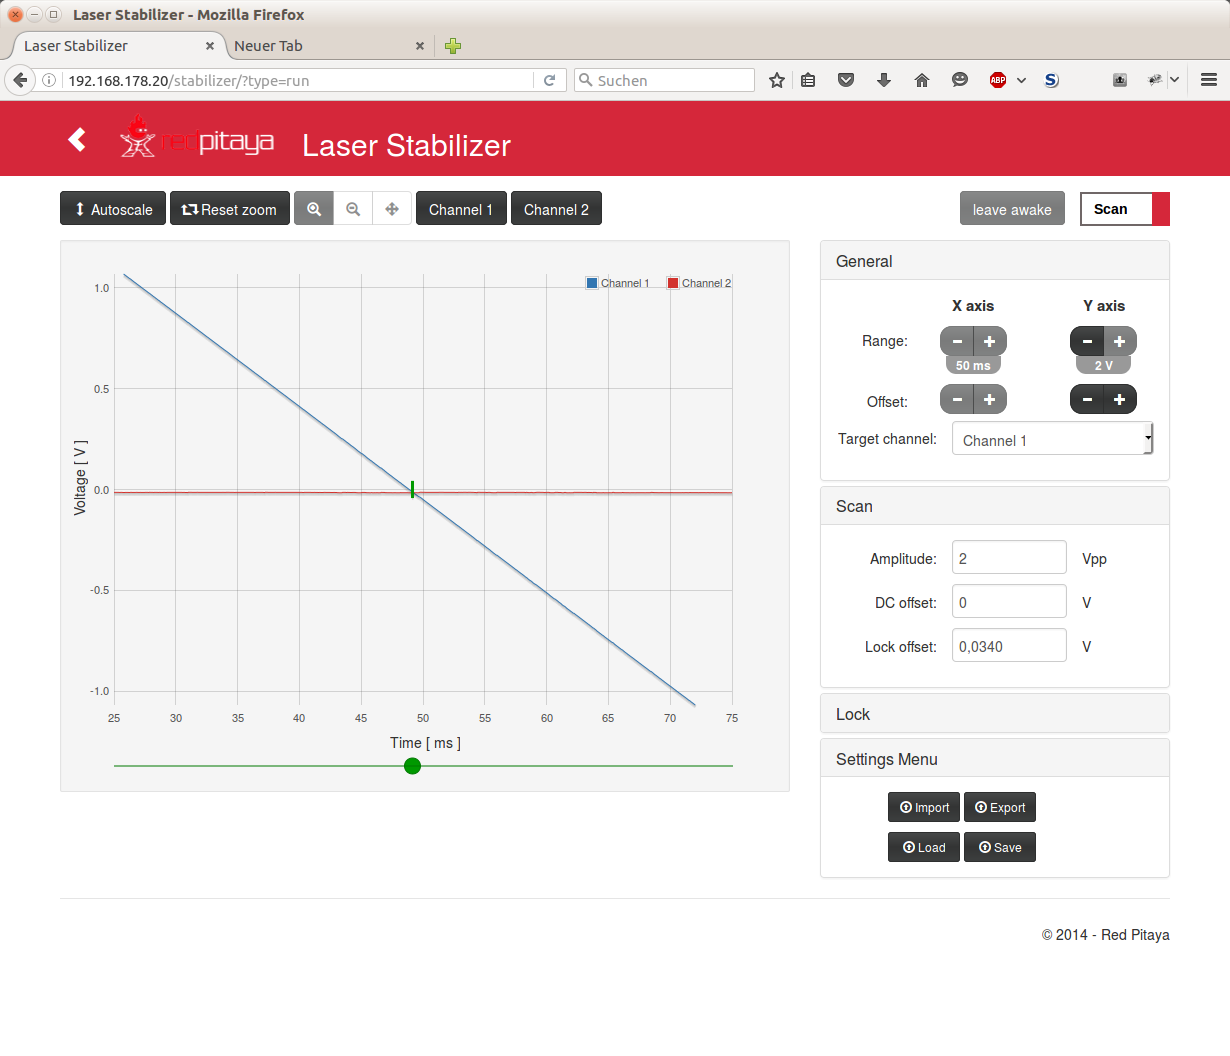
\includegraphics[width=0.9\textwidth]{stabilizer.png}
	Screenshot der Weboberfläche der Stabilizer App im \textbf{Scan Mode}
\end{figure}

Im \textbf{Scan-Mode} generiert die Stabilizer App ein 10Hz Dreieckssignal (Scansignal) variabler \textbf{Amplitude} an dem \textbf{Target-Channel} und misst die anliegenden Spannungen (Fehlersignale) an den beiden Input-Channeln über eine volle fallende Flanke. Mit einem Schieberegler kann nun eine Stelle im Fehlersignal markiert werden. Dabei wird der Zeitwert der x-Position in die dazu korrespondierende Spannung des Scansignals umgerechnet. Dieser \textbf{Lock-Offset} dient später als Spannungsoffset für die PIDs. Hat man eine passende Stelle im Fehlersignal gefunden und die PIDs konfiguriert, kann in den \textbf{Lock-Mode} umgeschaltet werden. Nun wird ein DC Offset mit Wert des \textbf{Lock-Offsets} an dem \textbf{Target-Channel} generiert und die PIDs gestartet. Im Lock-Mode können jetzt auch Änderungen an der Zeitbasis etc. vorgenommen werden. Außerdem lässt sich die App im \textbf{Lock-Mode} über die Schaltfläche \textbf{leave awake} ohne Beenden verlassen.\\
Im Menu \textbf{Settings} können die vorgenommenen Einstellungen exportiert oder auf dem RedPitaya gespeichert werden. Die gespeicherten Dateien werden dabei mit einem Erstellungsdatum versehen, sodass alte Dateien beim Speichern nicht überschrieben werden. Sie liegen auf dem RedPitaya im Verzeichnis \grqq /var/opt/stabilizer/\grqq~. Die dortige Datei \grqq settings\_meta\grqq~enthält den Namen der aktuellen Einstellungsdatei, sodass manuell durch Ändern der Meta-Datei alte Einstellungen wieder eingespielt werden können. Auch Importieren und Laden (der auf dem RedPitaya gespeicherten Daten) ist möglich.\\

Das gesamte Projekt findet sich unter \grqq web-apps/stabilizer/\grqq~in meinem Archiv.


\section{Nützliches}

\subsection{Exportieren von Dateien auf den RedPitaya (Ubuntu)}
Das Dateisystem des RedPitayas ist bis auf wenige Verzeichnisse wie \grqq /var\grqq~schreibgeschützt. Mit dem Befehl (per ssh ausführen) 'ro' und 'rw' wird das Dateisystem nicht-beschreibbar, bzw. beschreibbar. Auch sollte man bei Aktualisierungen innerhalb der Webanwendungen zuvor den WebServer mit 'systemctl stop redpitaya\_nginx.service' stoppen und anschließend wieder mit 'systemctl start redpitaya\_nginx.service' starten. Um mir das etwas zu vereinfachen, habe ich ein kurzes bash-Skript (für Linux) geschrieben:

\lstset{breaklines=true, showstringspaces=false, keywordstyle=\bfseries\color{purple},
commentstyle=\itshape\color{green},
identifierstyle=\color{blue},
stringstyle=\color{orange},basicstyle=\footnotesize\ttfamily}

\lstinputlisting[caption={rp\_push\_file.sh},captionpos=t,language=bash]{../bin/rp_push_file.sh}

\subsection{Schutz der laufenden Web-App vor versehentlichem Beenden}
Öffnet ein zweiter Nutzer eine schon laufende App, so kommunizieren beide Nutzer mit der selben \grqq Instanz\grqq~des Controller-Programms.\\
Startet er jedoch eine andere App, führt dies zum sofortigen Beenden der laufenden Anwendung. Im Falle von Anwendungen, die über längere Zeit laufen müssen, ist dies natürlich fatal. Leider zeigt das Hauptmenü der Weboberfläche des RedPitayas nicht an, ob eine, und wenn ja welche, Anwendung gerade läuft.\\

Um dieses Problem zu lösen, muss das Hauptmenü entsprechend angepasst werden, dessen Dateien im Verzeichnis \grqq /opt/redpitaya/www/apps/\grqq~auf dem RedPitaya liegen. Insbesondere die Datei \grqq index.html\grqq~und die darin verlinkten Javascript-Dateien müssen bearbeitet werden. Da die Weboberfläche sich für die verschiedenen Versionen des RedPitaya OS ändern kann, müssen die Änderungen bei einer neuen Versionen erneut und gegebenfalls abgändert vorgenommen werden. Glücklicherweise sollte folgendes Grundgerüst versionsunabhängig funktionieren:\\
\begin{enumerate}
\item Zunächst ist herauszufinden, welche und/oder ob eine App gerade läuft. Hierzu kann verwendet werden, dass eine laufende App auf eine Get-Anfrage an die Adresse 'root\_url' + '/data' antwortet. Erhält man eine Antwort, ist unmittelbar einsehbar welche App gerade läuft, da die Antwort deren Id enthält. Dieses Verfahren funktioniert allerdings nicht für Pro-Apps...
\item Nun kann z.B durch Einblenden einer Warnung auf eine evtl. laufende App reagiert werden.
\end{enumerate} 
Wie gesagt, muss diese Methode versionsabhängig implementiert werden, einige Implementierungen finden sich allerdings bereits im Verzeichnis\\\grqq web-apps/prevent\_user\_from\_killing\_apps\grqq~meines Archivs.

\section{Anhang}

\subsection{acq\_api\_test}
\lstset{breaklines=true, showstringspaces=false, keywordstyle=\bfseries\color{purple},
commentstyle=\itshape\color{green},
identifierstyle=\color{blue},
stringstyle=\color{orange},basicstyle=\footnotesize\ttfamily}

\lstinputlisting[caption={acq\_api\_test},captionpos=t,language=c]{../acq_api_test/main.c}

Das Programm produzierte die folgende Ausgabe:
\begin{alltt}
\input{../acq_api_test/acq_api_test_output.txt}
\end{alltt}
\end{document}